\section{Questões de projetos referente a funções}
\begin{frame}{Questões de projetos referente a funções}
\begin{block}{Considerações}
	\begin{itemize}
	  \item Efeitos colaterais
	  \item Tipos de valores retornados
	  \item Quantidade de valores retornados
	\end{itemize}
\end{block}
\end{frame}

\begin{frame}[fragile]{Efeitos colaterais}
\begin{block}{Exemplo de aliasing}
	\begin{verbatim}
		int x = 3; 
		... 
		... // se int* y = &x;
		*y = 9;
	\end{verbatim}
\end{block}
\end{frame}

\begin{frame}{Tipos de valores retornados}
\begin{block}{Alguns exemplos}
	\begin{itemize}
		\item C permite qualquer tipo ser retornado por suas funções exceto vetores e funções. 
		\item C++ permite tipos definidos pelo usuário ou classes serem retornados. 
		\item Java e C\#, qualquer tipo ou classe podem ser retornados por seus métodos.
	\end{itemize}
\end{block}
\end{frame}

\begin{frame}[fragile]{Quantidade de valores retornados}
\begin{block}{Linguagem Lua}
	Lua permite o retorno de múltiplos valores de suas funções. Por exemplo, a chamada da função:
	\begin{verbatim}
		a, b, c = fun() 
	\end{verbatim}
	Recebe três valores de retorno da função func():  
	\begin{verbatim}
		return 3, sum, index
	\end{verbatim}
\end{block}
\end{frame}

\section{Sobrecarga de operadores definidos pelo usuário}
\begin{frame}[fragile]{Sobrecarga de operadores}
Linguagens como Ada, Python, Ruby e C++ suportam sobrecarga de operadores. 
\begin{lstlisting}
	CVector CVector::operator+ (CVector param) {
	  CVector temp;
	  temp.x = x + param.x;
	  temp.y = y + param.y;
	  return (temp);
	}

	int main () {
	  CVector a (3,1);
	  CVector b (1,2);
	  CVector c;
	  c = a + b;
	  cout << c.x << "," << c.y;
	  return 0;
	}
\end{lstlisting}
\end{frame}

\section{Closure} 
\begin{frame}[fragile]{Closure}
Closure é uma variável local em uma função que é mantida viva (não é desalocada) após o retorno dessa função. Linguagens como C\# e JavaScript possuem closure. 
\begin{lstlisting}
function foo(x) {
  var tmp = 3;
  return function (y) {
    alert(x + y + (++tmp));
  }
}

var bar = foo(2);
bar(10); 
\end{lstlisting}
\end{frame}

\section{Co-rotinas} 
\begin{frame}[fragile]{Co-rotinas}
Co-rotinas são um tipo especial de subprogramas. A linguagem Lua é uma das linguagens que possui co-rotinas. Geralmente, corrotinas são criadas pela aplicação por uma unidade chamada de unidade mestre.
\begin{figure}[ht!]
 \centering
 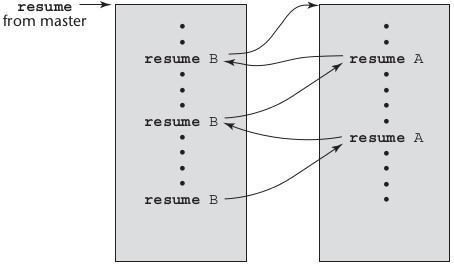
\includegraphics[scale=0.5]{./imgs/coroutines.png}
\label{co-rotinas}
\end{figure}
\end{frame}

\begin{frame}{Co-rotinas}
\begin{figure}[ht!]
 \centering
 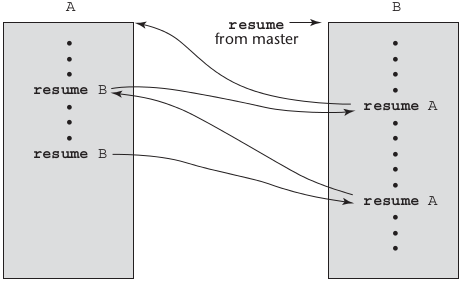
\includegraphics[scale=0.5]{./imgs/coroutines_b.png}
\label{co-rotinas_b}
\end{figure}
\end{frame}


